%%%%%%%%%%%%%%%%%%%%%%%%%%%%%%%%%%%%%%%%%
% University/School Laboratory Report
% LaTeX Template
% Version 3.1 (25/3/14)
%
% This template has been downloaded from:
% http://www.LaTeXTemplates.com
%
% Original author:
% Linux and Unix Users Group at Virginia Tech Wiki 
% (https://vtluug.org/wiki/Example_LaTeX_chem_lab_report)
%
% License:
% CC BY-NC-SA 3.0 (http://creativecommons.org/licenses/by-nc-sa/3.0/)
%
%%%%%%%%%%%%%%%%%%%%%%%%%%%%%%%%%%%%%%%%%

%----------------------------------------------------------------------------------------
%	PACKAGES AND DOCUMENT CONFIGURATIONS
%----------------------------------------------------------------------------------------

\documentclass[UTF8]{ctexart}

\usepackage{siunitx} % Provides the \SI{}{} and \si{} command for typesetting SI units
\usepackage{graphicx} % Required for the inclusion of images
\usepackage{graphics}%图片设置
\usepackage{subfigure} 

\usepackage{natbib} % Required to change bibliography style to APA
\usepackage{amsmath} % Required for some math elements 
\usepackage{amssymb} % 使用因为所以符号
\usepackage{fancyhdr} % 使用页眉

\usepackage{algorithm}
\usepackage{algorithmic}

\usepackage{listings} % 插入代码
\usepackage{xcolor}
\lstset{
    %backgroundcolor=\color{red!50!green!50!blue!50},%代码块背景色为浅灰色
    rulesepcolor= \color{gray}, %代码块边框颜色
    breaklines=true,  %代码过长则换行
    numbers=left, %行号在左侧显示
    numberstyle= \small,%行号字体
    %keywordstyle= \color{red},%关键字颜色
    commentstyle=\color{gray}, %注释颜色
    frame=shadowbox%用方框框住代码块
    }

%\usepackage{url} % 引用URL
% \usepackage{cite}
% \newcommand{\upcite}[1]{\textsuperscript{\textsuperscript{\cite{#1}}}} %参考文献上标

\pagestyle{fancy}
\fancyhf{} 
\cfoot{\thepage} 

\setlength\parindent{0pt} % Removes all indentation from paragraphs

\renewcommand{\labelenumi}{\alph{enumi}.} 

%----------------------------------------------------------------------------------------
%	DOCUMENT INFORMATION
%----------------------------------------------------------------------------------------
\title{算法分析与设计-作业四}

\author{王宸昊 2019214541}

\date{\today}

\begin{document}

\maketitle

%----------------------------------------------------------------------------------------
%	SECTION 1
%----------------------------------------------------------------------------------------

\section{CLRS, Page, 210 15.1-4}

\subsection{实现思路}

使用s[i]来记录切割点的坐标,在每次更新状态值时,记录相应的位置信息。\\
递归结束后,依次寻找切分点。\\

\subsection{实现代码}

\begin{lstlisting}[language={python}]
    # 动态规划-带备忘录的自顶向下方法-记录路径
    def Extended_Memoized_Cut_Rod(p, n):
        r = [-1] * (n + 1)
        s = [0] * (n + 1)  # 记录最优解路径
        Extended_Memoized_Cut_Rod_Aux(p, n, r, s)
        print(r)
        print(s)
        print("最优解:%d" % r[n])
        print("最优路线:")
        while n > 0:
            print(s[n])
            n = n - s[n]

    def Extended_Memoized_Cut_Rod_Aux(p, n, r, s):
        if r[n] >= 0:
            return (r[n])
        if n == 0:
            max_value = 0
        else:
            max_value = -1
        for i in range(1, n+1):
            temp = Extended_Memoized_Cut_Rod_Aux(p, n-i, r, s)
            if max_value < p[i] + temp:
                max_value = p[i] + temp
                s[n] = i    # 记录最优时切分点的位置
        r[n] = max_value    # 记录下n时的最小值
        
        return max_value
\end{lstlisting}

\subsection{输出结果}

\begin{figure}[H]
    \centering
    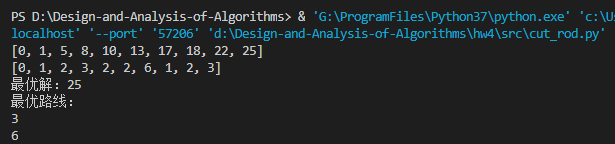
\includegraphics[width=1\textwidth]{img/res-1.png}
    \caption{不同规模下排序算法时间对比}
    \label{带切割方案的备忘录方法}
\end{figure}


%----------------------------------------------------------------------------------------
%	SECTION 2
%----------------------------------------------------------------------------------------

\section{CLRS, Page, 222 15.3-4}

证明:\\
假设现在有四个矩阵:$A_1, A_2, A_3, A_4$,输入的维度序列$ p = [1000, 100, 20, 10,1000] $。\\
Capulet教授的算法为贪心策略,每次选择使$p_0 * p_k * p_4$最小的k值。所以第一次选择k=3时,将矩阵乘法顺序变为$((A_1A_2A_3)A_4)$,第二步选择k=2,将顺序调整为$(((A_1A_2)A_3)A_4)$。总的乘法计算次数为$1000*100*20 + 1000*20*10 + 1000 * 10 * 1000 = 12,200,000$。\\

而当计算顺序为:$((A_1(A_2A_3))A_4)$时,总的乘法计算次数为$100*20*10 + 1000*100*10 + 1000 * 10 * 1000 = 11,020,000$。\\

由此可见,只采用贪心的策略可能会得到次优解。
  
%----------------------------------------------------------------------------------------
%	SECTION 3
%----------------------------------------------------------------------------------------

\section{基于接缝裁剪的图像压缩}

\subsection{证明}
假设在第i行的接缝数量为$S_i$,由算法原理可知,在第i-1行中的接缝位置一定在其上方或者左上或者右上,除了左右边界以外,对每行的接缝都有3种可能。因此此时的接缝可能数为$3^m$。假如在每行中都是边界,则接缝的可能数是$2^m$。综上,接缝的数量是m的指数函数。

\subsection{算法原理}
假设输入的图像为M*N大小。\\
首先先定义$d[i, j]$表示删除像素$A[i, j]$的对图像的破坏度,破坏度越低,与相邻像素的相似度越高。这里我们使用Energy Map来表示破坏度,能量图一般使用图像像素的梯度取模,为了简化计算,可以先将RGB三通道转为单通道的灰度图,其次,不再对每个像素点进行求梯度,而是计算周围点的绝对值差,如下公式:
\begin{equation*}
    energy\_map[i][j] = \left\lvert img[i-1][j] - img[i+1][j] \right\rvert + \left\lvert img[i][j-1] - img[i][j+1] \right\rvert
\end{equation*}
$dp[i, j]$表示从第一行到第i行的最小破坏度,利用动态规划的思想找到一条使得从上到下最小破坏度的线,对于每一行的像素,向上一行八联通的三个点中,选取dp最小的点,更新当前的dp值。dp的更新策略如下:
\begin{equation*}
    dp[i][j] = energy\_map[i][j] + min(dp[i-1][j-1], dp[i-1][j], dp[i-1][j+1])
\end{equation*}

接下来将找到的这条直线删除,在某一方向上就去掉了一个单位的线,重复以上的过程即可缩放图片。

\subsection{伪代码}
\begin{algorithm}[H]
	\caption{CHOOSE\_MIN$(dp, i, j[], n)$}   %算法标题
    \begin{algorithmic}[1]  %一行一个标行号
       
        \IF{$n\leq1$}
        \RETURN{n}
        \ENDIF
        \RETURN{FIB\_RECUR(n-1) + FIB\_RECUR(n-2)}
        
	\end{algorithmic}
\end{algorithm}

\subsection{算法效果}
编译环境为Python3.7,操作系统的版本为Windows 10。\\
CPU为AMD Ryzen 7 1700(3.0 GHz),RAM 16G。\\
第三方模块:
\begin{itemize}
\item time(): 对算法执行过程进行高精度的计时,最高精度可达微秒级别
\item random(): 产生任意大小的随机数
\item sys():查看内存使用情况
\end{itemize}

\subsection{实验结果}


\begin{table}[H]
    \caption{$10^9$输入规模下算法性能测试}
    \label{table-1}
    \begin{center}
        \begin{tabular}{cc}
            \hline
            排序算法&   执行时间(s)\\     
            \hline
            快速排序&       13510.133\\               
            归并排序&       17861.703\\              
            希尔排序&       23620.192\\             
            基数排序&      9998.141\\                      
            \hline
        \end{tabular}  
    \end{center}
\end{table}

从上表的数据可以明显的看出,从总体上看,在数据量比较大的时候,排序是一件相当耗时的事情。以快排为例,进行一次排序约3.7个小时。同时可以看出,在基于比较的算法的当中,快速排序的算法的执行时间是最优秀的,基数排序作为一种接近线性的算法,其执行时间明显优于其他基于比较的算法,在10进制的情况下,只需要2.7个小时就可以完成排序。

\end{document}